
\documentclass{sig-alternate-10pt}
%\documentclass{sig-alternate-05-2015}
\usepackage{algorithm}
\usepackage{algorithmicx}
\usepackage{pifont}
\usepackage{algpseudocode}
\usepackage{color}
\usepackage{cite}
\usepackage{bm}
\usepackage{subfigure}
\usepackage{makecell}
\usepackage{balance}
\usepackage{url}
\usepackage{breakurl}
\usepackage{bm}
\usepackage{graphicx}
\usepackage{subfigure}
\usepackage{multirow}
\usepackage{makecell}
\usepackage{float} 

\begin{document}


\title{DronEar: Drone Privacy Invasion Detection System \\ Based on Audio}

\numberofauthors{1} %  in this sample file, there are a *total*
% of EIGHT authors. SIX appear on the 'first-page' (for formatting
% reasons) and the remaining two appear in the \additionalauthors section.
%
\author{
Youcheng Liye, Jiawei Xu
\\
\email{\{liye97, xujiawei\}@whu.edu.cn}
\and %\\
       \affaddr{The State Key Lab of Software Engineering, School of Computer Science, Wuhan University, P. R. China}\\
       }

\maketitle

%\hspace{20mm}
\begin{abstract}

With the development of technology, consumer-level drones are increasingly popular among hobbyists and recreational use. But the increased usage also rises concerns about privacy issues. Without physical access, attackers can control the drone to fly over fences and walls to observe the interior of  house or fly to a certain height to observe the conditions in high-rise windows, posing a threat to personal privacy and business secrets. 

In this work we propose DronEar, a new type of drone detection system that uses inexpensive, off-the-shelf commercial microphones to receive the noise from drone propellers and process it to achieve drone detection and the prevention of privacy intrusion. We defined an attacker model and decompose the action of drone into four types of primitives. The algorithm we designed based on RSSI and formant diagram is used to analyze the sound of drone to judge its current state.

We tested our system using three popular consumer drones. The results show that our system can stably extract the sound characteristics of the drone and effectively detect the existence of drone, and also recognize the motion state of drone. If a drone is about to cause privacy invasion, our system could send out a warning to the user, inform them to making further preventions.


\end{abstract}


\keywords{ Drone, RSSI, Spectrogram }

\section{Introduction}
\subsection{Background}
Consumer drones has gained its popularity nowadays. Since the launch of Parrot AR. Drone in 2010, the use of these devices is no longer restricted to military and commercial domains nor enthusiasts, but has opened up to laymen as well. At the same time, the continuous development of sensors and image processing technology as well as the increasing perfection of flight-assist features makes drone easily accessible to hobbyists. This is further supported by the popularity of smart phones and tablets, which provides a convenient operating platform for consumer drones. Drone manufacturers are launching more affordable and feature-rich products every year, and the number of drones for video and entertainment uses is increasing: In 2015, global sales of consumer drones were about 1.3 billion dollars. IDC (International Data Corporation) estimates that by 2020, the market size will reach 3.7 billion dollars, and the market will ship more than 4 million units by then. At the same time, as an emerging product, drones still have some technical, regulatory, and social barriers, and controversial issues related to public safety and privacy arise during unmanned operations.

But this prevalence of consumer drones is not without risks. Over the past few years incidents at high-security facilities have occurred with increasing frequency. Outside the prison, drones were used to deliver contraband, weapons, mobile phones. Drug smugglers use drones to transport goods to the border. Under the watch of the White House Secret Service, a drone operated by a drunken American government employee, rushed into the South Lawn of the White House in night.

In addition to the above-mentioned dangers caused by drones entering restricted areas, the general public is increasingly uneasy about the intrusion of privacy by drones carrying high-fidelity camera equipment. Since most consumer-grade drones can transmit live video during flight, they can fly over fences into nearby open spaces to capture and transmit private images and data, and even view indoors through windows, potentially threatening to the privacy of individuals and institutions. A father in Kentucky, suspected that a drone flying over a neighbor's yard was spying at his daughter who was sunning and using a shotgun to shoot it down; a man in Xi'an used a drone to shoot a woman at home, lived the naked scene and broadcast it.
 
These and similar incidents have prompted reactions from regulators. The FAA (Federal Aviation Administration) will be centered on most airports and the radius of 5 miles will be designated as “No Fly Zone”, The drones cannot take off in this area. If the drones in the flight break into the area, they will also be forced to land. At the same time, many tourist attractions and national parks are also included in the no-fly zone. DJI has also set up the no-fly zone of protected areas for their product, including the vast majority of airports in the world. The FAA also requires that since December 2015, the owner of the drone must be registered as a drone operator to legally use the drone; the Civil Aviation Administration of China has issued the Regulations on the Registration of the Real-name System of Civil Unmanned Aerial Vehicles, announced that since June 2017, the purchase of drones weighing more than 250 grams must be real name registered. In this way, if the drone is harmful, it can be traced back to the individual according to the registered information and punished accordingly. In addition, most countries and institutions set the default maximum flying height of the drone to 120 meters, which prevents the drone from harming large aircraft such as airplanes.

In this work, we propose a system that detects the presence of a consumer drone with sound during drone flight. In the real environment, we tested the robustness of the drone detection system in different flight modes, flight speeds and noise environments.

In doing so we made the following specific contributions:
\begin{itemize}
\item The algorithm can detect drone sound that is uniquely differentiated from other small flying objects, such as birds and insects.
\item Development of a model of drone-based privacy invasion attacks.
\item Reporting the evaluation of our system in a real-world scenario using popular consumer drones.
\item Proposal of mechanisms to overcome attempts by an attacker to avoid detection, such as mute the drone or modify the vocal frequency of the drone propeller.
\end{itemize}
\section{ Audio Signatures and Basic Movements of Drones}
DronEar relies on the unique audio signatures produced by drone propellers to detect drone presence and its movements, as well as differentiate them from other noise making objects.  In this section, we start by providing the background of spectrogram and drone audio signatures, then discuss four basic movements of drones and how their audio signature shifts as they move.
\subsection{Drone Audio Signatures}
Our project works by setting up an omni-directional microphone in a privacy-sensitive place to pick up the sound of surrounding drones, and by extracting, analyzing, and processing the audio information, to determine the motion state of the drone around the subject. Infer whether the current subject is under the threat of illegal piracy by the intruder operating the drone.

The main features in the audio information from the microphone we extracted include: RSSI (Received Signal Strength Indication) of the sound signal, and logical position information of the resonance peak of the sound signal, including the time of occurrence and the frequency where it located.

In the features above, the RSSI value of the sound signal objectively reflects the signal strength of the sound emitted by the drone received by the microphone: the larger the RSSI value, the greater the signal strength of the sound emitted by the drone received by the microphone, which indicated the drone is closer to the microphone; the smaller the RSSI value, the smaller the signal strength of the sound from the drone received by the microphone, and indicates drone is farther from the microphone. Based on this, we can use the “Distance-Detecting Sectional Type Algorithm Based on RSSI” we designed to approximately calculate the distance between the drone and the microphone that receives the sound. 

\begin{figure*}[!t]
	\centering
	\subfigure[Relative RSSI when drawing near]{
		\label{rssi near}
		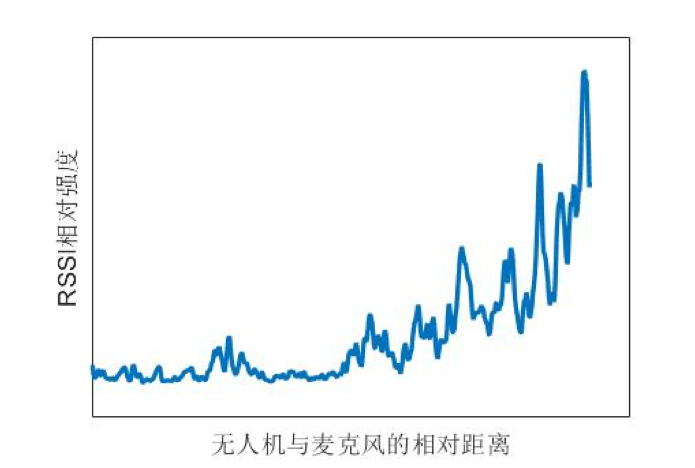
\includegraphics[width=0.4\textwidth]{pics/rssi_near.png}}
	\subfigure[Relative RSSI when moving away]{
		\label{rssi far}
		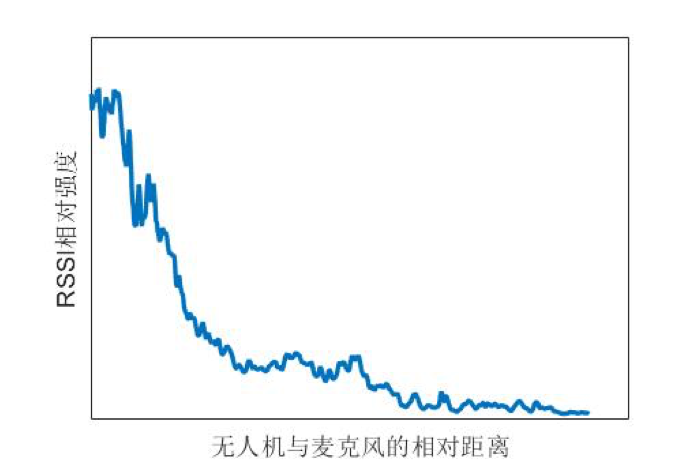
\includegraphics[width=0.4\textwidth]{pics/rssi_far.png}}
	\caption{Relations between RSSI and drone movements}
	\label{rssi}
\end{figure*}

The resonance peak proposed by us in the features above is actually a reference to the concept of resonance in the field of speech recognition, and is a term of acoustic phonetics. In the field of speech recognition, a resonance is a reinforced speech band that is displayed on a spectrogram automatically drawn by a sound spectrograph. When the sound passes through the resonant cavity, it is filtered by the cavity, so that the energy of different frequencies in the frequency domain is redistributed, part of which is strengthened by the resonance of the resonant cavity, and the other part is attenuated. Because the energy distribution is not uniform, the strong part comes more significantly than the weak part, then it is called "resonance". In our project, the concept of resonance is similar. We perform a short-time Fourier transform on the sound information from the drone received by the microphone, and we will obtain a sound intensity-frequency distribution map at each sampling instant. By setting the formant intensity threshold parameter $\beta_{strength}$, we filter out the sound frequency whose sound intensity is higher than the formant intensity threshold parameter $\beta_{strength}$ for the sound intensity-frequency distribution at each sampling time, that is, the logical position information of the formant of the sound signal received by the microphone is extracted. 

\begin{figure}[!h]
	\centering
	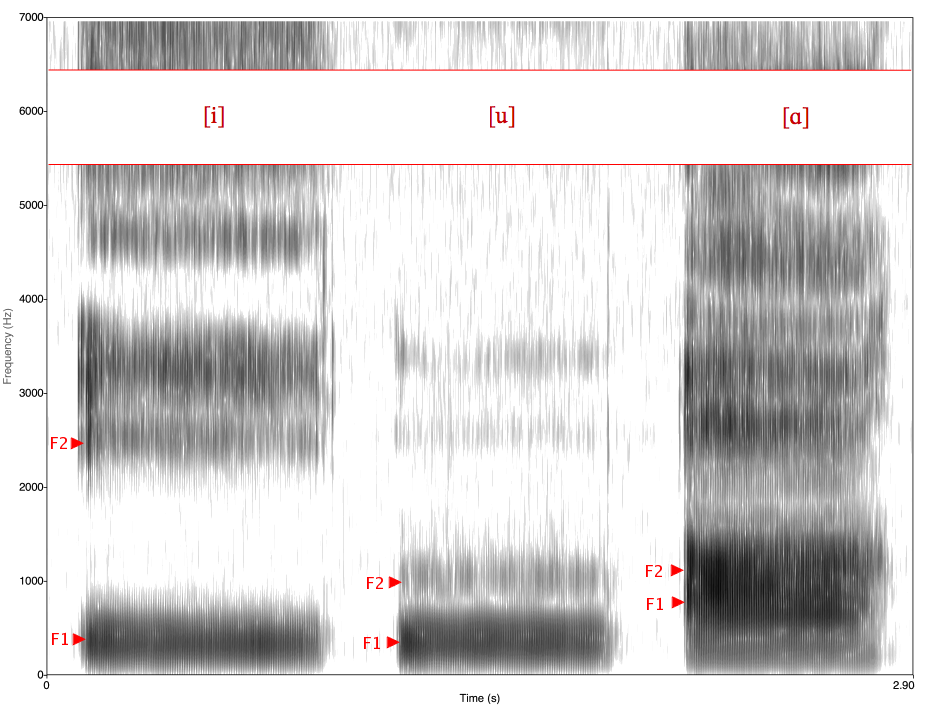
\includegraphics[width=0.4\textwidth]{pics/spectrogram.png}
	\caption{Spectrogram of voice}
	\label{spec}
\end{figure}


\subsection{Drone Movements}
In the drone intrusion model we envisioned, the intruder used an unmanned aerial vehicle to invade the privacy or trade secrets of other individuals, attempting to violate the subject's wishes and to capture images inside the building. In this model, we assume that the intruder does not have the ability to modify the commercial unmanned aerial vehicle that they used, and they control the original unmanned aerial vehicle they purchased to complete the invasion.

Since the unmanned aerial vehicle controlled by the intruder for intrusion cannot enter the interior of the building, the intruder must first control the drone to move it near a certain window outside the building during the completion of the intrusion. ZCP (Zone of Comfortable Photographing), in which the drone can capture pictures in the windows of the building more clearly and steadily. As shown in Figure \ref{zcp}, this action can be split into two parts: raising the drone vertically to a level of the window and moving the drone horizontally towards the window. After completing the actions above, the drone is in the shooting comfort zone outside a certain window of the building, and the intruder often tries to adjust the distance of the drone to the window (near or away) to obtain a suitable angle of view. and suitable The clarity of the shooting until they can clearly use the drone to capture the picture they want. However, it is worth noting here that the drone cannot be arbitrarily approached to the outside of the building or its window. When the drone is very close to the outside of the building or its window, the instability of the airflow near the side of the building will result in an imbalance of airflow around the drone, which will make the drone difficult to control and increase the intrusion failure. risk.
\begin{figure}[!h]
	\centering
	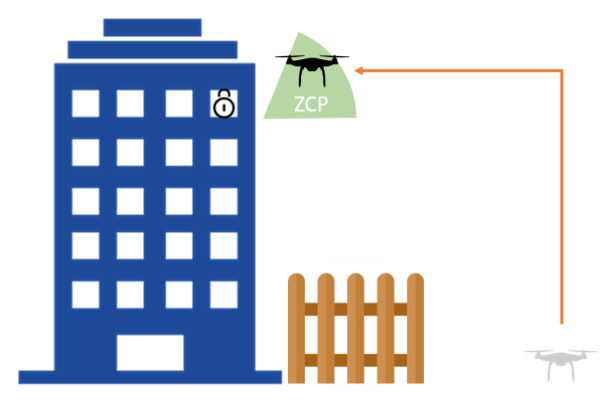
\includegraphics[width=0.4\textwidth]{pics/zcp.png}
	\caption{A typical privacy invasion attack by drone}
	\label{zcp}
\end{figure}

\begin{figure}[!h]
	\centering
	\subfigure[Moving up]{
		\label{up}
		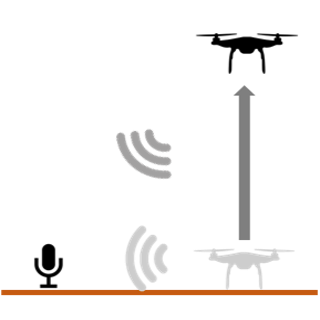
\includegraphics[width=0.2\textwidth]{pics/up.png}}
	\subfigure[Moving down]{
		\label{down}
		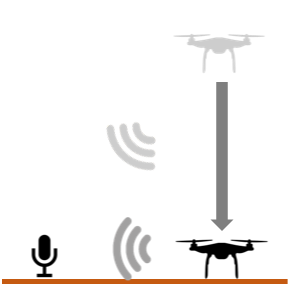
\includegraphics[width=0.2\textwidth]{pics/down.png}}
	\subfigure[Moving near]{
		\label{near}
		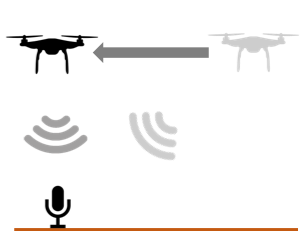
\includegraphics[width=0.2\textwidth]{pics/near.png}}
	\subfigure[Moving away]{
		\label{far}
		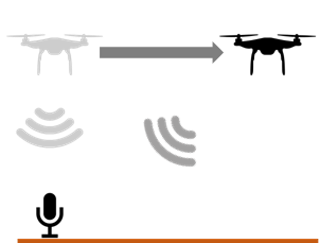
\includegraphics[width=0.2\textwidth]{pics/far.png}}
	\caption{Four basic types of movements of drone}
	\label{movements}
\end{figure}

\section{System Design}

The DronEar proposed by us continuously receives the sound information of the surrounding environment through the microphone in real time, and judges whether there is a drone in the surrounding environment. if there is a drone, it continues to judge the movement of the drone and detects whether there is a drone intrusion threat under the current situation.
A number of algorithms are introduced in order to capture and analyze the presence and movements of the drone.
In the following subsection, we first define our problem and identifies challenges in realizing such a system, then introduce three main modules of our system and how they cooperate with each other to form a pipeline-like system. We then present the detail of the algorithm we designed and explain how they realize in detecting ranges and movements.

\noindent{\textbf{Challenges.}}However, 

\begin{enumerate}
	\item \textbf{Computing speed.}
	
	\item \textbf{Computing speed.} Because the algorithm used to extract the audio features is complicated, and the processing time is longer than the time of the audio itself. In order to solve this problem, we need to enable parallel computing when processing audio. In addition, the number of samples can be reduced by reducing the sampling rate of the drone audio to reduce the amount of calculation.
	\item \textbf{Feature extraction.} When the distance of microphone and drone is getting further, the vocal feature we received becomes less noticeable, which means same movement degree of drone would result in fewer feature changes. This limits the maximum detection range of our system.
	\item \textbf{Environment noise.} When the drone is far away from the microphone, the environmental noise has a great impact on the audio acquisition and processing of the drone, so we applied noise canceling to the sound signal we received to overcome the impact of environmental noise.
\end{enumerate}

\subsection{Problem Formulation}


\subsection{Modules}

 The real-time system is divided into three modules, which work together to operate in a pipeline-like manner. The three modules are:
\begin{itemize}
    \item Data acquisition module. The module is responsible for recording the sound detected by the external hardware device, the microphone, according to the specified sampling interval, and generating the corresponding audio file.
    \item Feature analysis module. The module is designed for analyzing the audio files generated by the previous module, and extracting corresponding features to determine the specific actions of the drone in the audio file of the previous module.
    \item Display module. The module is used for displaying the UAV’s action results analyzed and judged by the previous module to the user through the user interface, so that the user can see at a glance the current state of operation of the drone. Also, when a possible drone intrusion threat occurs, the module warns the user against possible UAV intrusion threats.
\end{itemize}
\begin{figure}[!h]
	\centering
	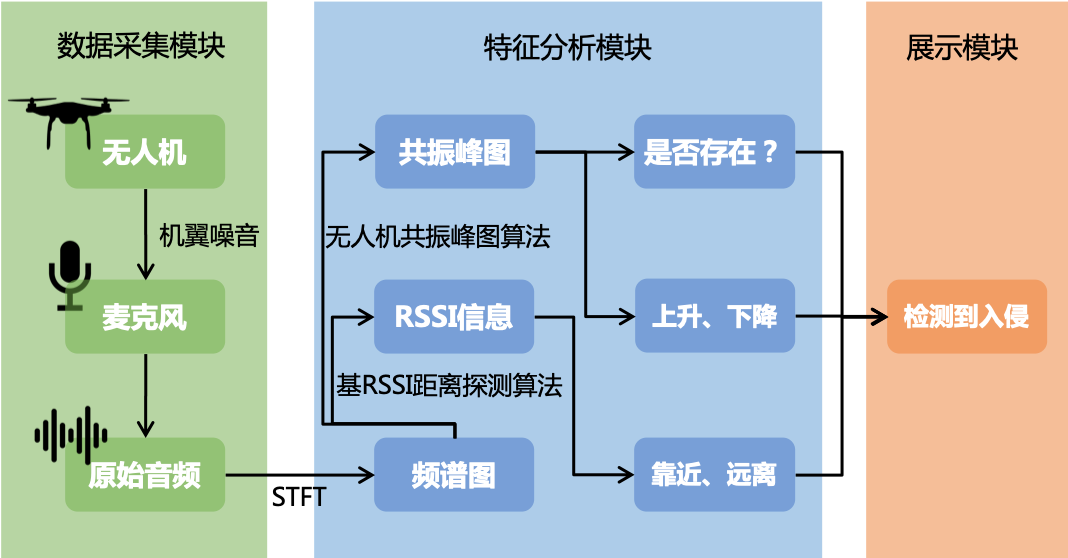
\includegraphics[width=0.45\textwidth]{pics/workflow.png}
	\caption{DronEar workflow}
	
	\label{workflow}
\end{figure}
The workflow of the system is as follows: after receiving the start command, the system starts to collect the sound signal in the environment and input it into the data analysis module for calculation and processing, and then determines the next action according to the processing result. If no drone is detected, return to the first step to continue collecting sound signals in the environment; if detected, continue to use our proposed base RSSI distance detection algorithm and UAV formant diagram algorithm to extract its action Information and compare it against our attacker model to detect whether it has malicious intrusion. If there is, the system will issue an alarm to prompt the user to take corresponding measures to avoid the risk; if not, continue to detect whether the drone still exists, and then continue to extract its action information for analysis and continuously monitor whether it is malicious; if not If it exists, go back to the first step and re-acquire the sound signal in the environment.


\subsection{Drone Movement Detection Algorithm}
In this section, we present DronEar's detection algorithms.
\subsubsection{Segmented distance detection based on RSSI}
The input of the algorithm code is a piece of mono audio signal $x(t)$. After a short time Fourier transform, the spectrum of the audio is obtained:
$$SP_x(t,f)=|X(t,f)|^2=|\int_{-\infty}^\infty\omega(t-\tau)x(\tau)e^{-j2\pi f\tau}d\tau|^2$$
Then the data on the sampling points on each spectrogram is modulo and summed:
$$rssi_i=\sum_{j=1}^n|data_{(i,j)}|$$
Get a matrix with only one row of stored results:
$$rssi=(rssi_1,rssi_2,......,rssi_n)$$
Each summation result is then subtracted from the result of the first two seconds, the result is compared to a predetermined threshold, and the result is stored in the result matrix:
$$
result_i = \left\{ \begin{array}{ll}
1 & \textrm{$rssi_1-rssi_{i-2}>threshold$}\\
0 & \textrm{$threshold>rssi_1-rssi_{i-2}>-threshold$}\\
-l & \textrm{$rssi_1-rssi_{i-2}<-threshold$}
\end{array} \right.
$$
$$result=(result_3,result_4,......,result_t)$$
\subsubsection{Drone formant diagram algorithm}
The input of the algorithm code is a piece of mono audio signal $x(t)$, and after a short time Fourier transform, the spectrum of the audio is obtained:
$$SP_x(t,f)=|X(t,f)|^2=|\int_{-\infty}^\infty\omega(t-\tau)x(\tau)e^{-j2\pi f\tau}d\tau|^2$$
Then, for each sampling point of the obtained spectrogram, the formant information on the sampling point is extracted by using a smooth spline function, and the resonance peak set at each sampling point is recorded as:
$$formant_1,formant_2,......,formant_t$$
Then, the algorithm code uses a data structure - "Disjoint-set" Initially, each formant is a separate set. Combine the set of resonant peaks with similar distances by enumerating the formant pairs:
$$Union_i=(formant_{(x_1,y_1)},formant_{(x_2,y_2)}),$$
$$where\ distance(formant_{(x_1,y_1)},formant_{(x_2,y_2)})$$
$$=min\bigcup_{i,j=0}^k distance(formant_{(x_i,y_i)},formant_{(x_j,y_j)})$$
These merge operations for the collection are maintained by the data structure "Union Set". After all the merge operations are completed, the formant in the same set together form a curve, which is recorded as:

$$line_i=(formant_{(x_1,y_1)},formant_{(x_2,y_2)},......\\,formant_{(x_y,y_y)})$$



Analyze the curves that are valid in all the constituent curves, the average of the slopes of these curves:
$$k_{average}=\sum_{i=1}^n\frac{k_{{line}_i}}{n}$$
The magnitude change of the interval frequency of adjacent formants at successive moments can be approximated. Furthermore, we can introduce the change in the angle formed between the drone and the microphone.


\begin{figure*}[!ht]
	\centering
	\subfigure[Original spectrogram]{
		\label{original_formants}
		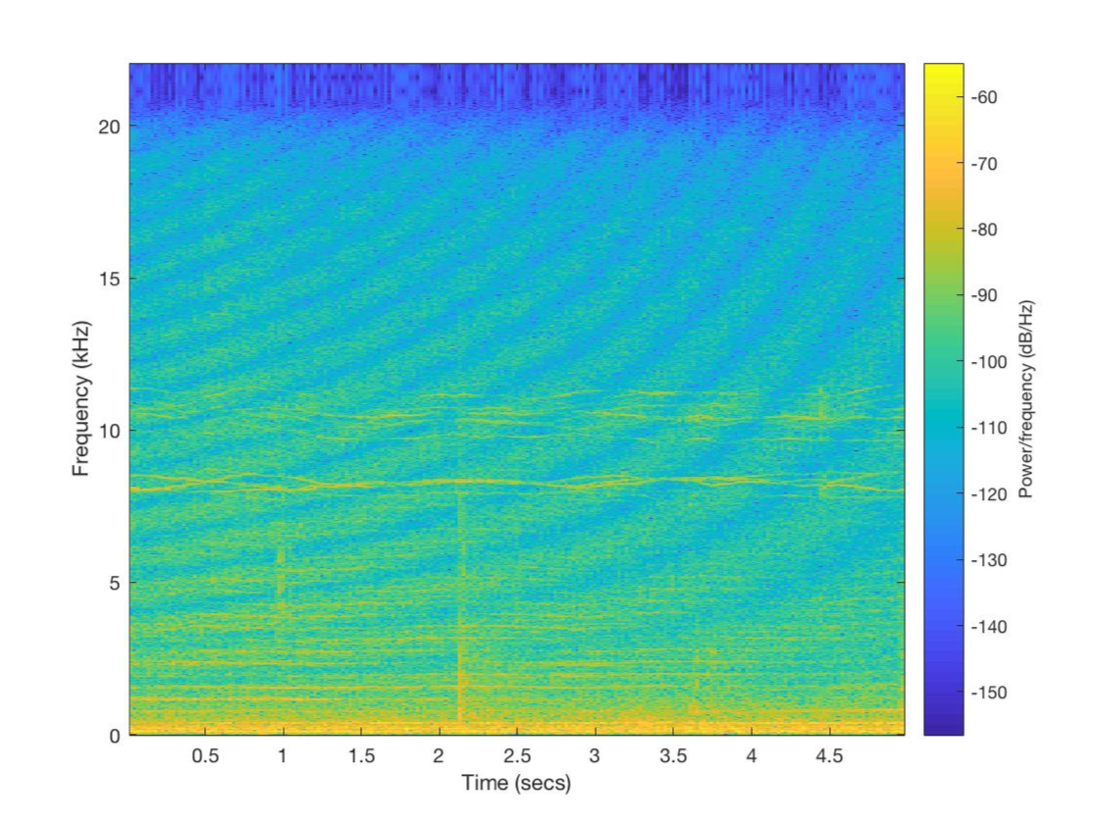
\includegraphics[width=0.3\textwidth]{pics/original_formants.png}}
	\subfigure[Locations of formants]{
		\label{processed_formants}
		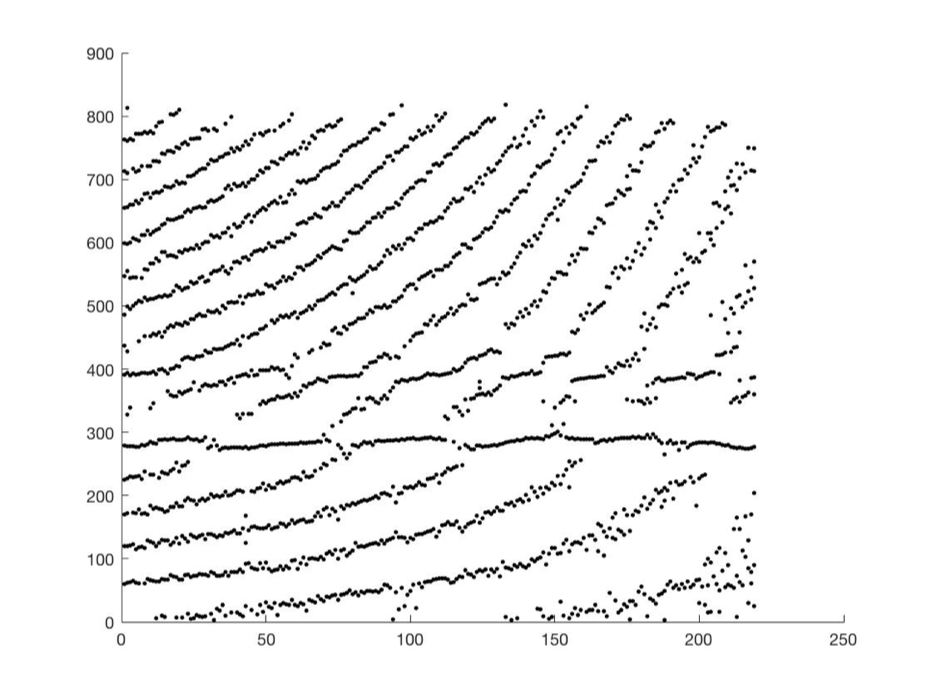
\includegraphics[width=0.33\textwidth]{pics/processed_formants.png}}
	\subfigure[Unioned formants]{
		\label{final_formants}
		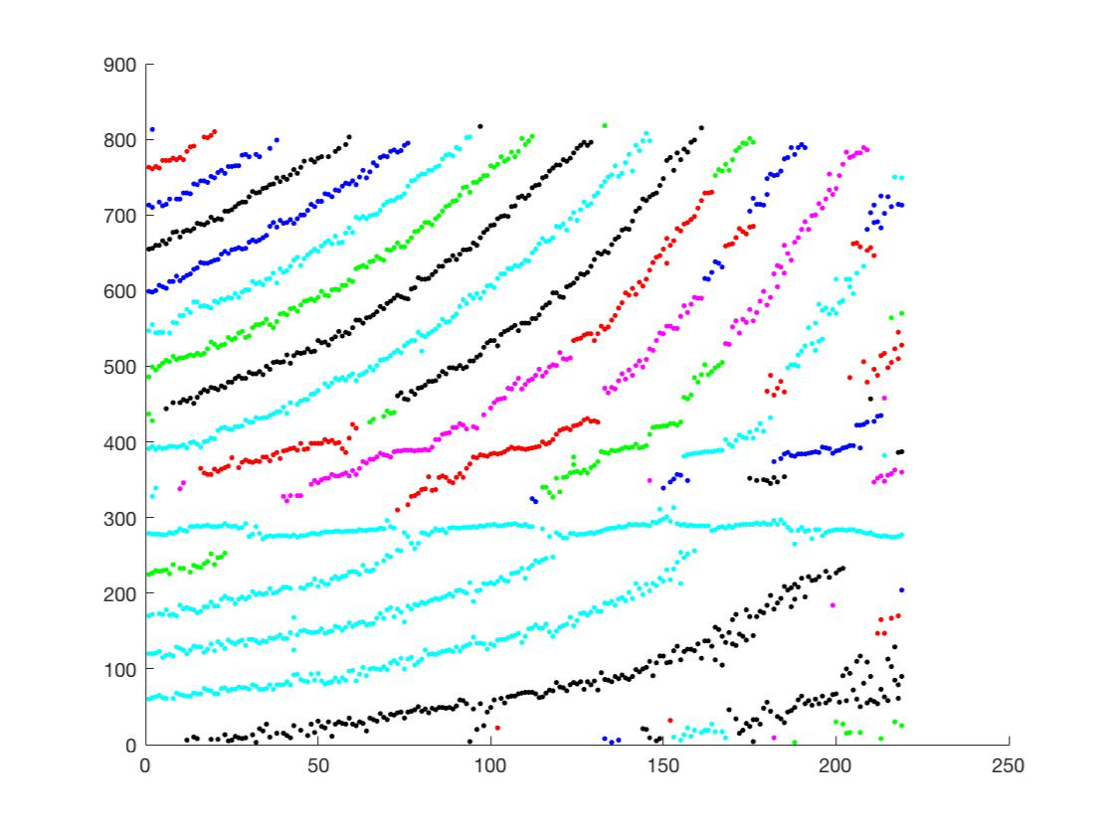
\includegraphics[width=0.33\textwidth]{pics/final_formants.png}}
	\caption{Processing of drone formants diagram algorithm}
	\label{formants}
\end{figure*}



\section{Evaluation}
\subsection{Experiment Setup}
\begin{figure}[!h]
	\centering
	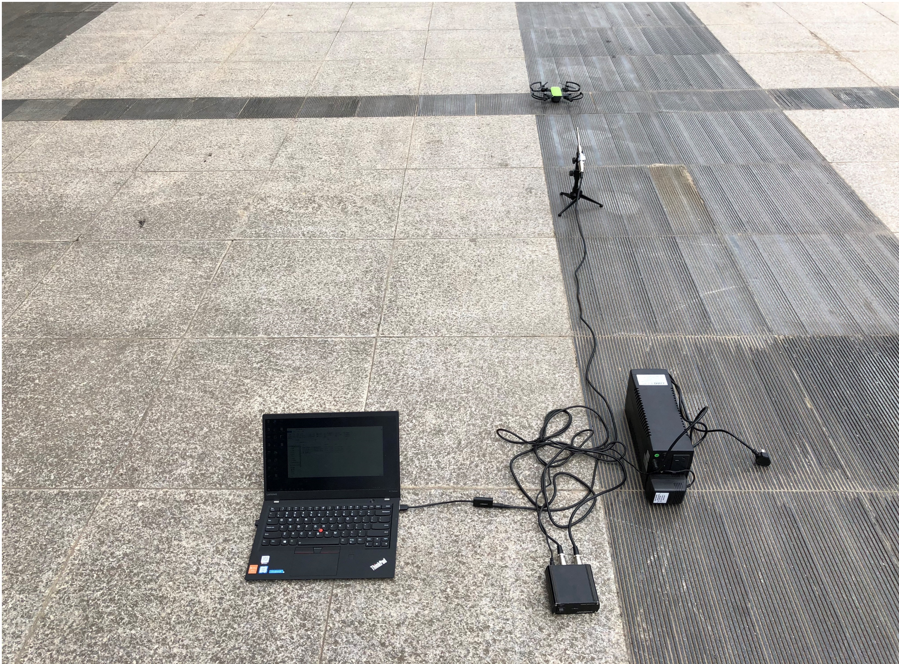
\includegraphics[width=0.4\textwidth]{pics/exp.png}
	\caption{Experiment equipments}
	\label{exp}
\end{figure}

We conducted experiments in three different environments, including a street next to the teaching building (as high noise environment) , athletic field (as ordinary noise environment) , top floor of the teaching building (as low noise environment) . In each environment, the data are collected when the drone is flying at different distances with respect to our receiver. We used three drones to conduct our experiment, including DJI Matrice M100, DJI Phantom 3 Advanced and DJI Spark to prove the robustness of our system to different drone models. 



\begin{figure}[!h]
	\centering
	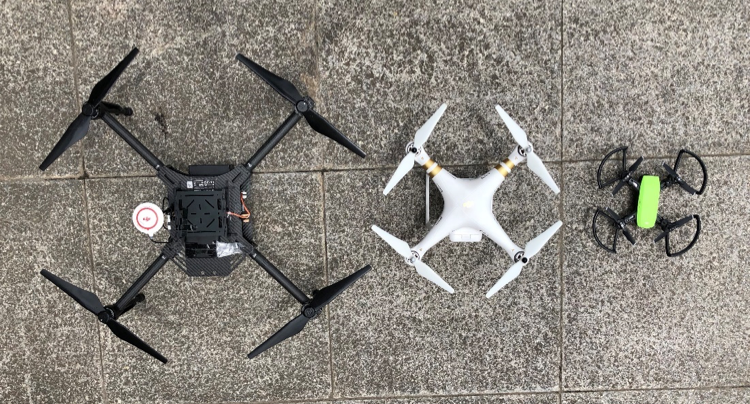
\includegraphics[width=0.4\textwidth]{pics/drones.png}
	\caption{Drones we used. From left to right, DJI Matrice 100, DJI Phantom 3, DJI Spark}
	\label{drones}
\end{figure}


\noindent{\textbf{Speeds.}}\hspace{1mm} 
We operate the drones in the different environments mentioned above at different flight speeds including slow speed, that the horizontal speed is less than 3m/s or the vertical moving speed is less than 1m/s. For this movement speed, the drone can keep its camera stable, suitable for recording and adjusting posture. Then medium speed, this state is the default normal speed of the drone flight. The horizontal speed is 3m/s~6m/s, or the vertical movement speed is 1m/s~2m/s. At this time, the drone camera is not easy to maintain in a stable state, suitable for short distance movement. Finally high speed, the state is a status after turning on the sport mode on drone. The horizontal speed is 6m/s or more, or the vertical moving speed is 2m/s or more. At this time, the camera is shaking violently, therefore, it is only suitable for long-distance movement.

\noindent{\textbf{Distances.}}\hspace{1mm} 
We also fly the drone at different distances, where the drone is initially 10 meters above the ground, and the drone moves up, down, close and away from the initial positions at a distance of five meters at six different initial positions from 5 meters to 15 meters away from the microphone every two meters. from the microphone to simulate the various situations that may be encountered in reality. The drone is controlled to take off and hover within the coverage area of the antenna receiver’s beam during all experiments.

In the experiment, we not only recorded the detection accuracy of the detection system (timely alarm feedback when the UAV invades and no false alarms when there is no UAV invasion) , but also accurately calculated the detection accuracy (the drone is detected by the detection system to detect the minimum distance of movement) under different conditions to find out the weakest link of the detection system and improve it.



\subsection{Result}



\section{Discussion}

Our system has focused on detecting the presence of drones through their loudness and frequency of the sound. We wish to expand our experiments to consider a wider variety of drones and greater distances Our system should be extended to contain anti-jamming devices for drone sounds from other sounding objects other than drones. Attackers may use this type of interference to cause our system to alert frequently. In this case, the user may reduce trust in our system or generate a kind of fatigue to the alarm, whichever is not conducive to privacy protection. Our system should also be enhanced to record the flight routes of intruding drones, localizing the position of the drone is the next logical step, but this consideration is outside the scope of this paper.


We would like to add a few microphones to experiment and try to get other aspects of the drone, not just his movements and existence, such as its precise position coordinates. 
We intend to add more action dimensions to the drone, such as hovering, and separate it from not moving.
We also desire to increase the processing speed of the system to make it more timely and capable. 
In addition, we wish to introduce more sound indicators into the algorithm to reach the point where the size of drone can be distinguished. 
Also in the future we hope to address the fact that our system is not currently capable of detecting multiple drones in the same vicinity at the same time. 
Moreover, we would like to evaluate the impact of different environments, e.g. windy condition, to the accuracy of detection. 
Finally, more experimental scenarios and drone privacy intrusion models need to be experimented to ensure the reliability of our systems.


\section{Related Work}
Multiple ways have been employed for drone detection, including radar, image and signal. We discuss these three ways respectively in this section.

\noindent{\textbf{Radar-based.}}\hspace{1mm} 
Radar is the traditional method of detecting aircraft. For a long time, it has been the main mean for military control of aircraft. But traditional radar systems cannot detect drones. In order to detect small objects such as drones, we must use expensive high-frequency radar systems, which is hard for individual users or small companies to use. In addition, Sanjay K Boddhu et al. believe that such radar systems are difficult to distinguish between birds and drones because they have the same wingspan. They proposed a method of using humans as sensors by a collaborative smart phone application that allows users to share information that the drone witnessed. Their approach is better suited to target large-scale threats and not to defend against a single target for nearby attackers.

\noindent{\textbf{Image-based.}}\hspace{1mm} 
Another way to detect drones is based on camera and image analysis. Rozantsev et al. detect small drones by using their appearance and motion characteristics. Busset et al. believe that the diversity of  shapes is challenging for appearance-based detection methods, and the motion-based approach is inconsistent with the similarities between UAVs and bird movements. Therefore, they recommend using an acoustic camera to complement the use of the camera. These microphone arrays use the noise of the rotor to detect the drone. Because they use dedicated and expensive equipment in the system, this is not a viable solution for use in a home or small business environment.

In addition, image-based detection methods require good lighting conditions to detect drones, which means that methods based on image detection of drones at night or in poorly lit areas will be difficult to apply, and this is  fatal for higher demand privacy protection. 

\noindent{\textbf{Signal-based.}}\hspace{1mm} 
Phuc Nguyen et al. proposed Matthan, a system that uses RF signals to detect the presence of drones. The system detects and processes the RF signal sent by drone in communication with the remote controller, and then detects the vibration and rocking characteristics of the drone to determine whether there is a drone within a certain range. Also based on communication signals between the drone and the remote control, Simon Birnbach et al. proposed a method of capturing video streams, because the video captured by the drone camera is transmitted to the screen of the remote control in real time. So analyzing the video stream to get the statistics of the drone movement and proximity to determine whether it is hostile is possible.

Peacock and Johnstone detect drones by using protocol signatures from drone Wi-Fi connections. For this to work, they must rely on unencrypted connections between the drone and the controller, but not for new models. They also discussed the use of media access control (MAC) address prefixes by known manufacturers to identify drones. Although this is a simple and reliable method of detecting a drone built by a manufacturer with a unique MAC prefix range, it can only detect known drone models, and with the drone model With more and more types, it is becoming more and more difficult to build and update a MAC prefix database. In addition, some manufacturers use uncertain MAC prefixes if their camera system on a drone includes a GoPro camera. But even when the drone manufacturer's MAC prefix is detected, relying on the presence of only certain MAC addresses is not sufficient to distinguish between the neighbors who are using the drone and the actual privacy intrusion attack.

Since the information they get comes from the communication between the drone and the remote control, when the attacker writes the motion path to the drone and automatically moves it around the target, the detection will fail. The purpose of privacy protection, in addition, the two methods above can only detect the presence or absence of the drone and cannot judge the motion state or trajectory of the drone, which has great limitations in the information dimension acquired.

\section{Conclusion}

The method based on sound instead of image for drone action and state detection is a non-contact drone recognition technology. Its advantages are as follows: The traditional UAV detection method usually uses GPS positioning system and radars, but radar is mainly used in military defense facilities, ordinary people can’t use it to detect the presence of potentially threatening drones within their range of activities. Traditional methods such as image recognition have the potential to confuse flying objects such as drones and normal birds. Compared with the above method, drone's sound signal for drone motion and condition monitoring is not affected by lighting conditions, and will not be confused by other flying objects similar to the drone. This makes our research on the flight state and action of invading drones by sound detection has an incomparable advantage compared with the traditional methods.

Based on the above, we propose an innovative algorithm for flight state and motion detection based on RSSI and Dijkstra. These two algorithms can complement each other. The RSSI algorithm mainly extracts the loudness characteristics of the sound emitted by the drone. The Dijkstra algorithm mainly extracts the number of formants. Theses algorithms make full use of the two most obvious characteristics of the loudness and frequency of the sound. Only one microphone captures a specific range of audio signals and transmits the signals to the computer. Using MATLAB to perform fast Fourier transform and other processing, the loudness variation and frequency distribution of all sounds in a short period of time can be obtained. Through the change of the acoustic sound level, it can be obtained whether the drone is currently close to or away from the user, and the number of formants is used to detect the presence of drones. The system has stable high recognition accuracy and great robustness.

At the same time, the experimental equipment used in our system is a very common and cheap equipment in daily life, easy to promote. The system we designed has broad application prospects. In addition, as an algorithm that relies only on sound to detect the presence and analysis of drones, our system can provide good scalability for future research on other dimensions such as images.

\bibliographystyle{acm}

\bibliography{sigproc}  
\end{document}